\documentclass[12pt]{article}
\usepackage{amsmath} % flere matematikkommandoer
\makeatletter
\renewcommand*\env@matrix[1][*\c@MaxMatrixCols c]{%
  \hskip -\arraycolsep
  \let\@ifnextchar\new@ifnextchar
  \array{#1}}
\makeatother
\usepackage[utf8]{inputenc} % æøå
\usepackage[T1]{fontenc} % mere æøå
\usepackage[danish]{babel} % orddeling
\usepackage{verbatim} % så man kan skrive ren tekst
\usepackage[all]{xy} % den sidste (avancerede) formel i dokumentet
\usepackage{listings}
\usepackage{graphicx}

\begin{titlepage}

\title{DBM 1}
\author{Christian Hohlmann Enevoldsen, MRB852}

\begin{document}
\maketitle

\end{titlepage}

{\setlength{\parindent}{0 cm}

\section{From ER to Relational}

1. 

Translation form ER to relational Schema \\\\
Stakeholders(\underline{CVR}, TEL, URL, Text) \\
Companies(\underline{\textit{CVR}}) \\
Owns(\underline{\textit{ownerCVR}, \textit{CVR}})\\
Municipalities(\underline{\textit{CVR}}, Budget) \\
Peope(\underline{Name}, Email, TEL) \\
WorkIn(\textit{CVR}, \textit{PersonName})\\
Project(\underline{PID}, Budget, URL) \\
Skills(\underline{Name})\\
NeedSkills(\underline{\textit{SkillName}, \textit{PID}}, PeopleCount) \\
HaveSkills(\underline{\textit{SkillName}, \textit{PeopleName}}) \\
Sponsors(\underline{\textit{PID}}, \textit{CVR})\\
Participate(\underline{\textit{StakeholderCvr}, \textit{PID}, Role})\\
Allocate(\underline{\textit{From}, \textit{To}, \textit{Percentage}, \textit{PersonName}, \textit{PID}}) \\\\
Den mest væsentlige ændring jeg har lavet i oversættelsen er at jeg har lavet statementet en attribute, da jeg ikke synes at en weak relation var nødvendig. Statementet bliver alligevel fjernet med stakeholderen. På samme måde kunne man bruge mapping oversættelse på det hele for at optimere databasen. Jeg har også valgt at fjerne periods, da allocate alligevel bruger de samme værdier som keys. \\ 

2.\\

CREATE TABLE Stakeholders (\\
  CVR CHAR(8) PRIMARY KEY,\\
  TEL CHAR(8) UNIQUE,\\
  URL VARCHAR(255) UNIQUE,\\
  Text VARCHAR(255) NOT NULL\\
);\\

CREATE TABLE Companies (\\
   CVR CHAR(8) PRIMARY KEY REFERENCES Stakeholders(CVR)\\
);\\

CREATE TABLE Owns (\\
  OwnerCVR CHAR(8) REFERENCES Stakeholders(CVR),\\
  CVR CHAR(8) REFERENCES Stakeholders(CVR),\\
  PRIMARY KEY (OwnerCVR, CVR)\\
);\\

CREATE TABLE Municipalities (\\
  CVR CHAR(8) PRIMARY KEY REFERENCES Stakeholders(CVR),\\
  Budget REAL\\
);\\

CREATE TABLE People (\\
  Name VARCHAR(35) PRIMARY KEY,\\
  Email VARCHAR(255) UNIQUE,\\
  TEL VARCHAR(8) UNIQUE\\
);\\

CREATE TABLE WorkIn (\\
  CVR CHAR(8) REFERENCES Stakeholders(CVR) NOT NULL,\\
  PersonName VARCHAR(35) REFERENCES People(Name) NOT NULL\\
);\\

CREATE TABLE Project (\\
  PID INT PRIMARY KEY,\\
  Budget REAL,\\
  URL VARCHAR(255) UNIQUE\\
);\\

CREATE TABLE Skills (\\
  Name VARCHAR(50) PRIMARY KEY\\
);\\

CREATE TABLE NeedSkills (\\
  SkillName VARCHAR(50) REFERENCES Skills(Name),\\
  PID INT REFERENCES Project(PID),\\
  RequiredPeople INT,\\
  PRIMARY KEY (SkillName, PID)\\
);\\

CREATE TABLE HaveSkills (\\
  SkillName VARCHAR(50) REFERENCES Skills(Name),\\
  PID INT REFERENCES Project(PID),\\
  PRIMARY KEY (SkillName, PID)\\
);\\

CREATE TABLE Sponsors (\\
  PID INT PRIMARY KEY REFERENCES Project(PID),\\
  CVR CHAR(8) REFERENCES Stakeholders(CVR) NOT NULL\\
);\\

CREATE TABLE Participate (\\
  CVR CHAR(8) REFERENCES Stakeholders(CVR),\\
  PID INT REFERENCES Project(PID),\\
  Role VARCHAR(255),\\
  PRIMARY KEY (CVR, PID)\\
);\\

CREATE TABLE Allocate (\\
  FromDate DATE,\\
  ToDate DATE,\\
  Percentage REAL,\\
  PersonName VARCHAR(35) REFERENCES People(Name),\\
  PID INT REFERENCES Project(PID),\\
  PRIMARY KEY (FromDate, ToDate, Percentage, PersonName, PID)\\
);\\
\\

3.

INSERT INTO Stakeholders (CVR, TEXT) VALUES ('21212121', 'Some text');\\

INSERT INTO Companies (CVR) VALUES ('21212121');\\

INSERT INTO Stakeholders (CVR, TEXT) VALUES ('42424242', 'Another text');\\

INSERT INTO Companies (CVR) VALUES ('42424242');\\

INSERT INTO Owns(OwnerCVR, CVR) VALUES ((SELECT CVR FROM Companies WHERE 
Companies.CVR = '42424242'\\),\\
                                         (SELECT CVR FROM Companies WHERE Companies.CVR = '21212121\\'));\\

INSERT INTO Project(PID, URL, Budget) VALUES (42, 'http://42.com', 100000);\\

INSERT INTO Sponsors(PID, CVR) VALUES ((SELECT PID FROM Project WHERE Project.PID = 42),\\
                                      (SELECT CVR FROM Companies WHERE Companies.CVR = '21212121'\\));\\


INSERT INTO Skills (name) VALUES ('Computer Programming');\\

INSERT INTO NeedSkills(SkillName, PID, RequiredPeople) VALUES (\\
  (SELECT name FROM Skills WHERE Skills.name = 'Computer Programming'),\\
  (SELECT PID FROM Project WHERE Project.PID = 42),\\
  42\\
);\\

4.\\

UPDATE Project\\
SET Budget=420000\\
WHERE Project.Budget = 100000;\\

\section{Relational Algebra}

1. $\pi_{names}(\sigma_{type=enzymes})(Proteins) $

2. $\pi_{Proteins.name}( \sigma_{name = TP53}(Gene) \times (Influences \times Protein) )$

3. $\pi_{ ( ( Proteins.id, type=enzyme )  \times (Infuences \times Gene \times (\sigma_{ type=membrane}(Protein))) ) }$

3. \pi_{pid} (\pi_{gid, pid}(\sigma_{type=enzyme}()))

\section{ER Modelling}

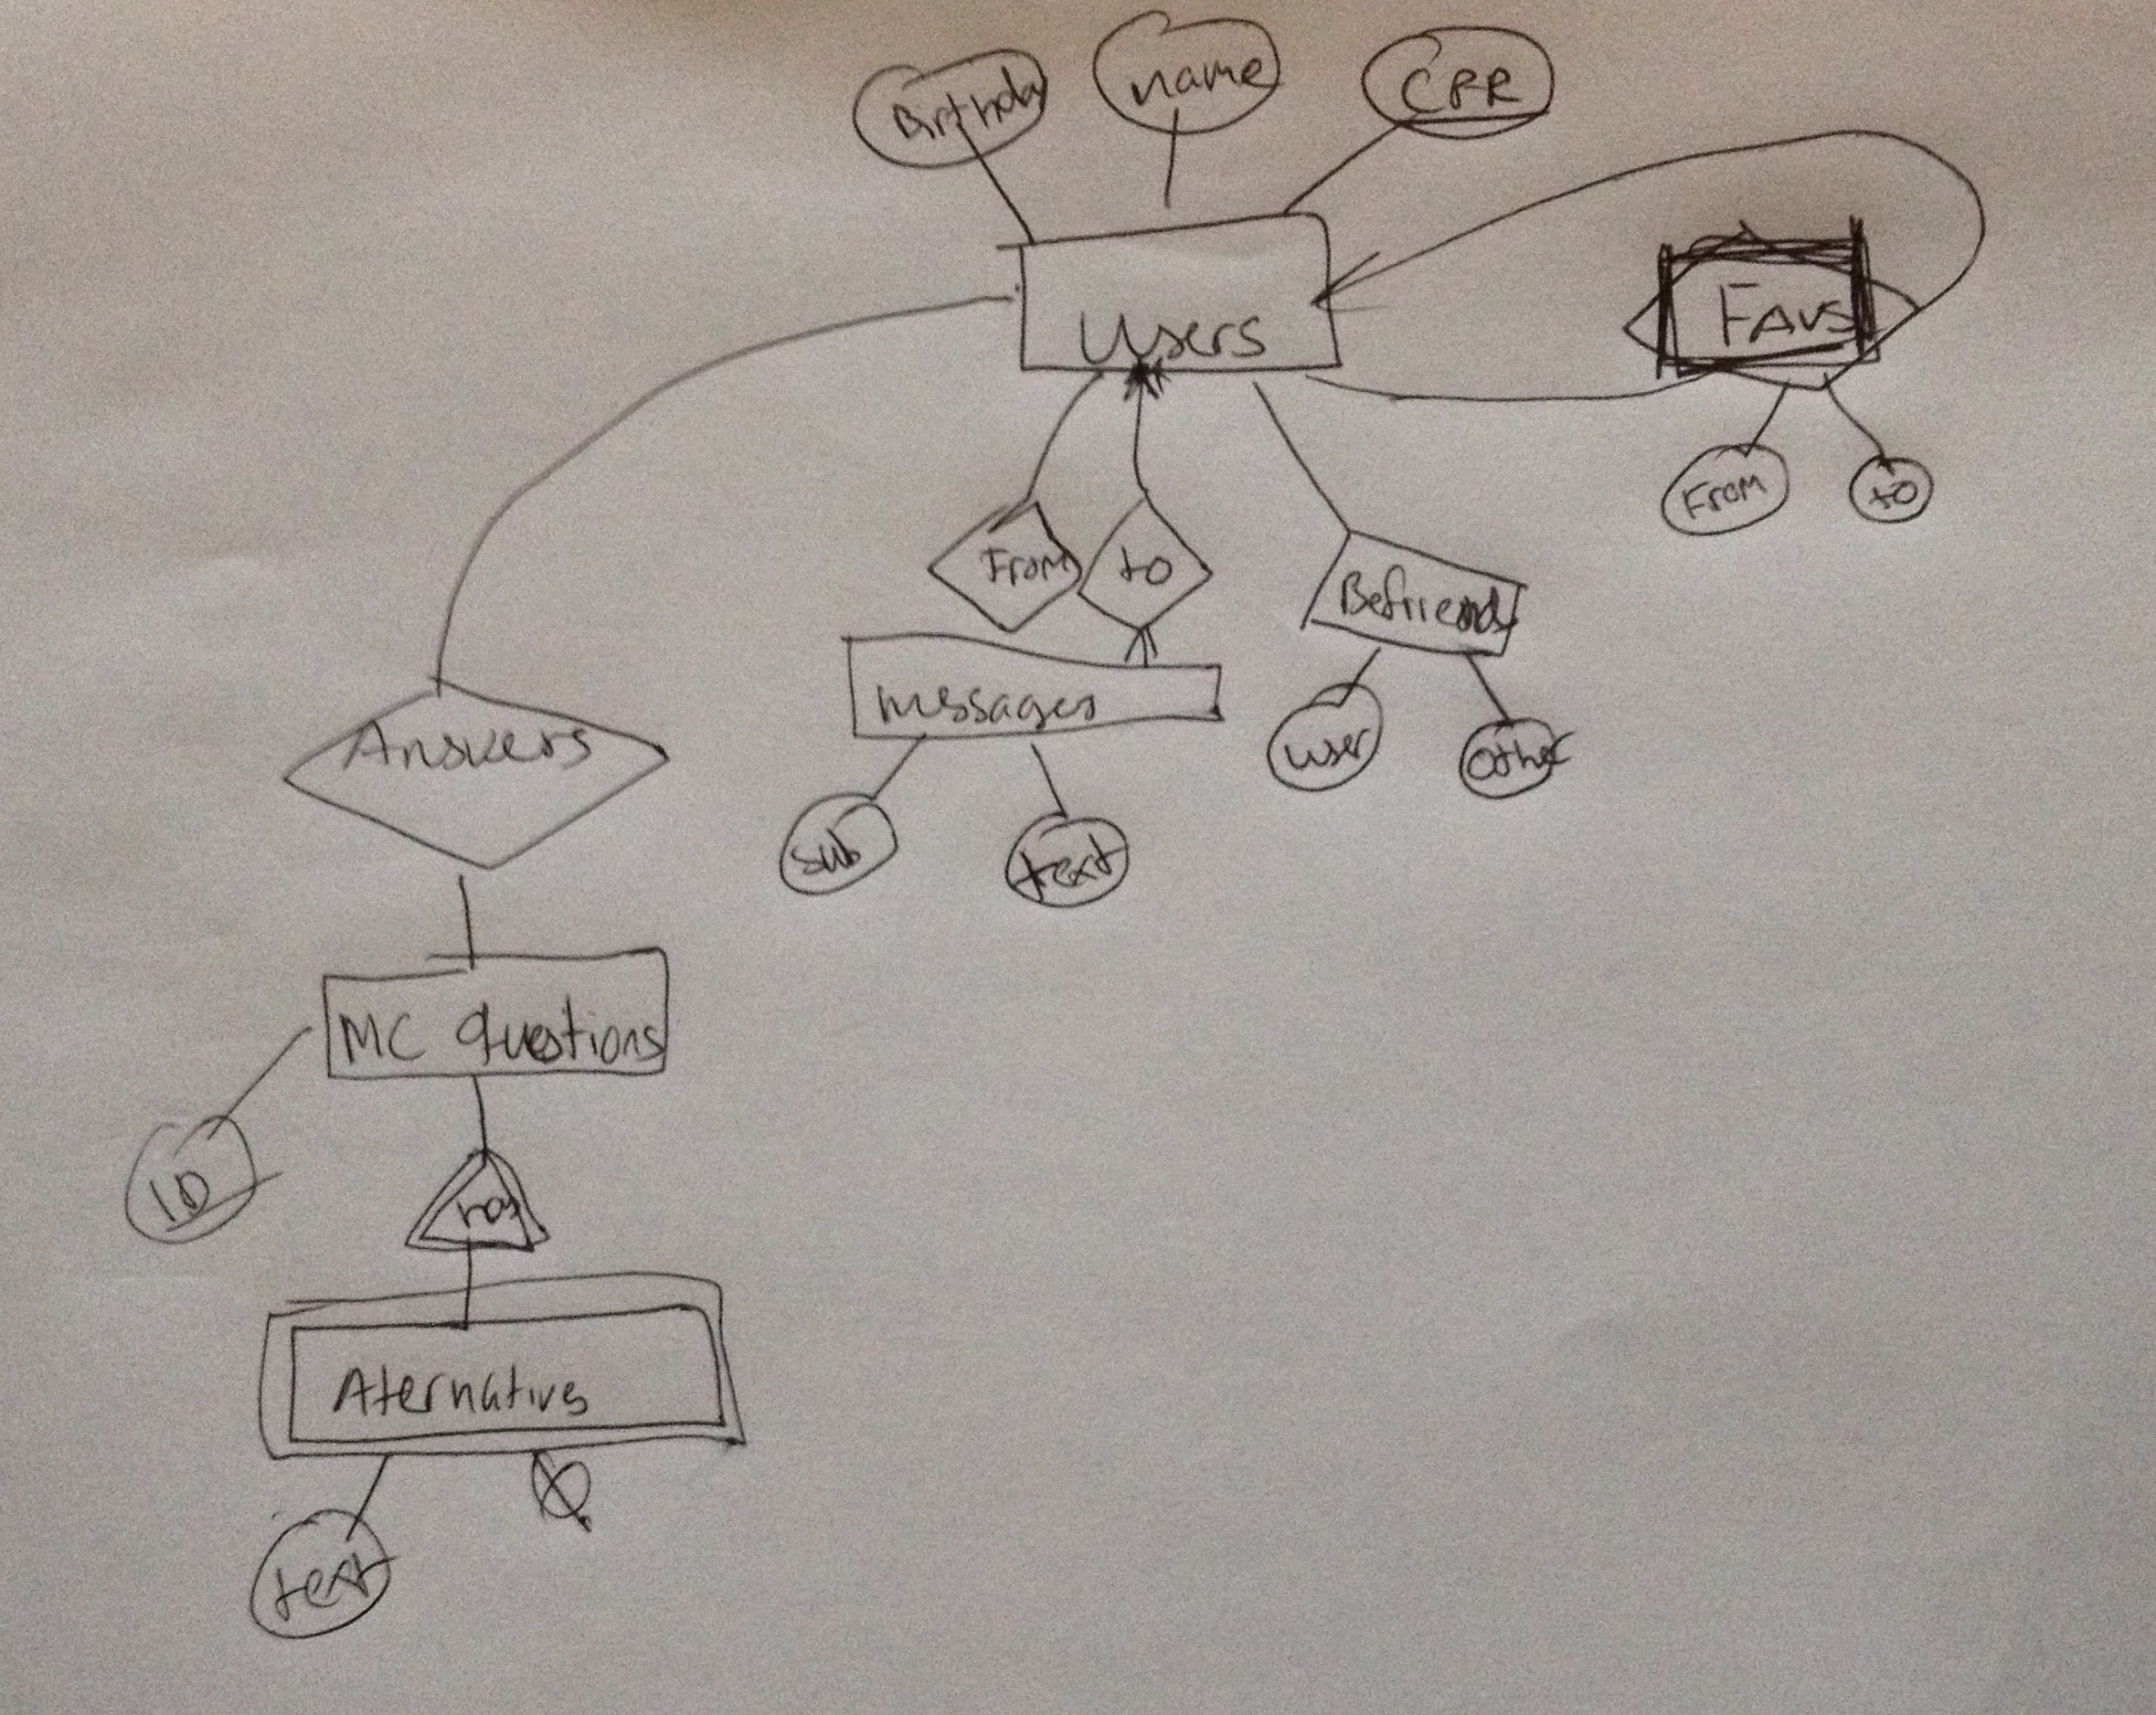
\includegraphics[scale=0.2]{photo.jpg}\\

Jeg har valgt at lave alternatives weak da der ikke er nogen primary key og uden questionarries vil det ikke give nogen mening at have dem.

\section {Functional Dependencies, Schema Design, and Normal Forms}

\section {SQL}

1.

SELECT names FROM proteins WHERE type=fibrous

2.

SELECT g.name\\
FROM Genes AS g\\
LEFT JOIN Influences AS i ON g.id = i.gid\\
RIGHT JOIN Protein AS p ON p.id = i.pid\\
WHERE p.type = 'membrane' AND p.type 'fibrous'\\

3. 

SELECT * \\
FROM Proteins AS p\\
LEFT JOIN Influences AS i ON\\
p.id  = i.pid \\
RIGHT JOIN Genes AS g ON g.id = i.gid\\
WHERE g.name IS 'TP53' AND g.name IS NOT 'BCO2'\\

4.

SELECT * \\
FROM proteins AS p \\
LEFT JOIN influences AS i ON p.id = i.pid \\
RIGHT JOIN genes AS g ON g.id = i.gid \\
HAVING COUNT(i.pid) > 42;\\


}



\end{document}

